% -*- mode: latex; mode: linkd; mode: auto-fill; mode: flyspell;-*-
\chapter{Design and Implementation}
\label{chap-five}


% Introduction

% Discuss what this chapter will focus on and dive in.
The purpose of this chapter is three fold: it discusses the motivations
that governed the design of the system, such as using the
BioBike\cite{journals/bioinformatics/MassarTES05} chassis and using
frames as a data structure to represent ACT-R based cognitive models;
it describes the work flow of the system that enables users to build
and share models and finally it discusses in detail a medium scale
model that was built as a proof of concept.

\section{Problem Definition for Coglaborate}

% This is where I have to discuss what coglaborate is trying to
% achieve 

The primary goal of the Coglaborate system is to provide a
collaborative tool-based environment for the computational cognitive
modeling community. Currently there are no known environments that
provide this facility. Apart from providing collaboration, Coglaborate
also intends to achieve a number of secondary goals:

% Sand boxing 
% Resource sharing
% Tool integration
% Knowledge agglomeration
\begin{itemize}
\item \emph{A sand boxed environment}: Currently there are number of
  interesting extensions to ACT-R. But occasionally it might be
  difficult for the users of the extensions to set them up. But with a
  sand boxed environment, users can connect to it and use the module
  with out any setup. This has a number of advantages, firstly the
  users do not have to keep track of the version of the extension and
  they can focus on completing their tasks rather than having to
  tinker around the computer.
\item \emph{Resource Sharing}: When we refer to resource sharing we refer to
  sharing hardware. With a web based platform that runs on a powerful
  computer researchers can simulate models that require excessive
  computational power and time.
\item \emph{Tool Integration}: If there are computational tools that a model
  would like to utilize they can be hooked in. For example the R
  statistical environment can be accessed by hooking in a
  library. Once loaded in a number of users would be able to access
  the facilities provided by it.
\item \emph{Knowledge Agglomeration}: As users model various aspects
  of cognition we would be able to build a repository that reflects
  the state of the field.
\end{itemize}

\section{Design Decisions}
% Design Decisions
%       - Why biobike
There were two major decisions that influenced the design of the
project: firstly the use of the BioBike chassis as a platform to
mount the ACT-R framework; and secondly the use of frames as means to
represent ACT-R based cognitive models in the shared memory. This
section discusses the alternatives that were analyzed and the reasons
why we chose to stick with the existing decisions.

\subsection{BioBike}

% Bio bike and the vision that it is originally based on
BioBike is an instantiation of
KnowOS\cite{oai:CiteSeerXPSU:10.1.1.75.7132} a concept based on the
view that knowledge could be treated on par as the rest of the
elements that make up a computer system. It is well known fact that
Operating systems provide abstractions to work with the elements of a
system for example, consider a file. An operating system provide
operations using which this file can be renamed, copied, deleted
etc. It also provides further abstractions that allow us to significant
modifications to raw data. The KnowOS vision extends this analogy to
the realm of knowledge. An implementation of the KnowOS consists of
the following layers\cite{oai:CiteSeerXPSU:10.1.1.75.7132}:


\begin{itemize}
\item An knowledge base centered around the frame system
\item An efficient and highly extensible language that provides an
  abstraction to the users to work with the system
\item A web-based interface to the programming language and to other
  KnowOS services.
\end{itemize}

% Description of biobike
%       - Components
BioBike originally known as BioLingua seeks to provide biologists with
the ability to perform computational biology operations on large data
sets using a simple language. BioBike ties up a number of knowledge
bases transparently using a frame based representation to represent
organisms. Being an implementation of the KnowOS vision it provides
features customized for molecular biologists. These include\cite{journals/bioinformatics/MassarTES05}

\begin{itemize}
\item A common framework to access genomic, metabolic and experimental data.
\item A general purpose programming language(lisp) customized to
  provide transparent access to the underlying knowledge bases.
\item A highly interactive environment where code can be evaluated and
  its results displayed immediately.
\item A number of general purpose tools that help in analyzing interactions.
\item A wiki through which scientists can collaborate and announce results.
\end{itemize}

% Talk about the style of interaction and the result
The BioBike language is built on top of Common Lisp. Users interact
with the system using a lisp listener. This results in a Unix style
interaction between the system and the user, where the user types in a
command and can see the results of that action immediately. All
listeners of the system share the same workspace as a result they can
share code.


\subsection{Frames}
%       - Why frames
% Brief description of other possible structures if I had not used frames.
%       - Semantic Nets
%       - Ontonlogies
%       - Frames
%       - Productions

\section{System Design}

\begin{figure}[htp]
  \centering
  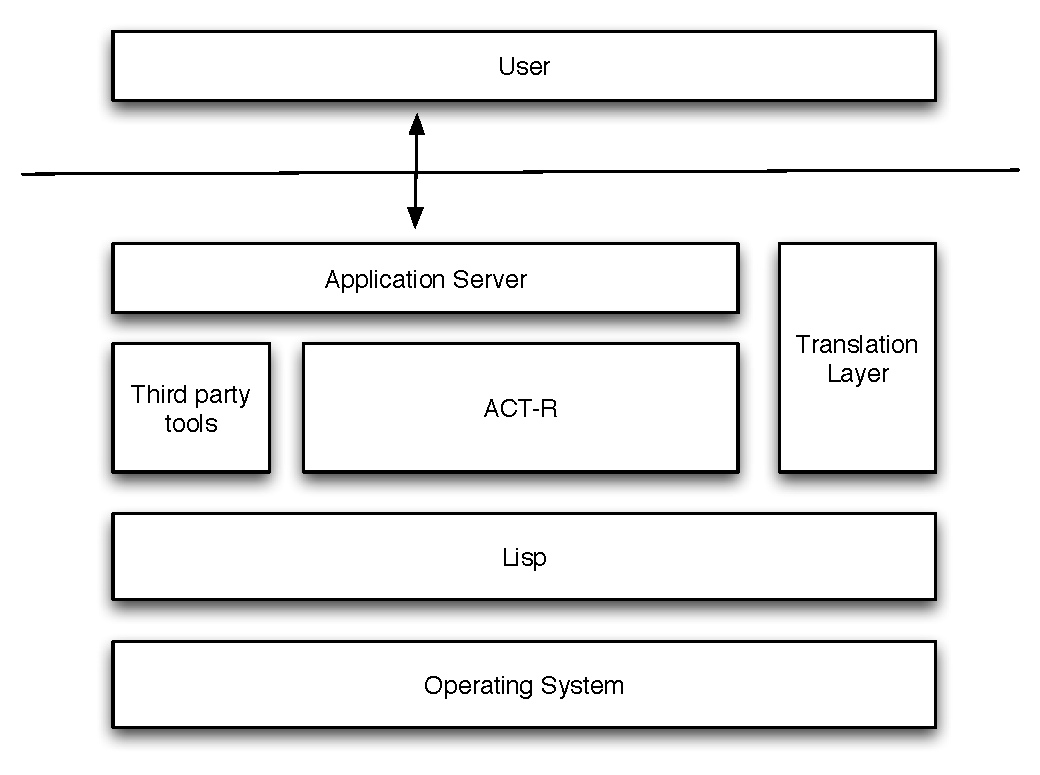
\includegraphics[width=90mm]{SystemOverview.eps}
  \caption{System Design}
  \label{SysOverview}
\end{figure}


\section{Work Flow}
% Coglaborate
%       - Describe work flow that shows collaboration occurs with screen shots.
%       - Describe what was modified and why
%         - Describe how frames are created
%         - Describe how the reverse procedure is implemented

\section{Proof of concept}
% Proof of concept
%        - Problem description
%        - Approaches
%        - Approach taken
%        - What can be deduced from it.

